\documentclass[border=10pt]{standalone}
\usepackage{tikz}
\usetikzlibrary{arrows.meta, shapes.geometric}

\begin{document}
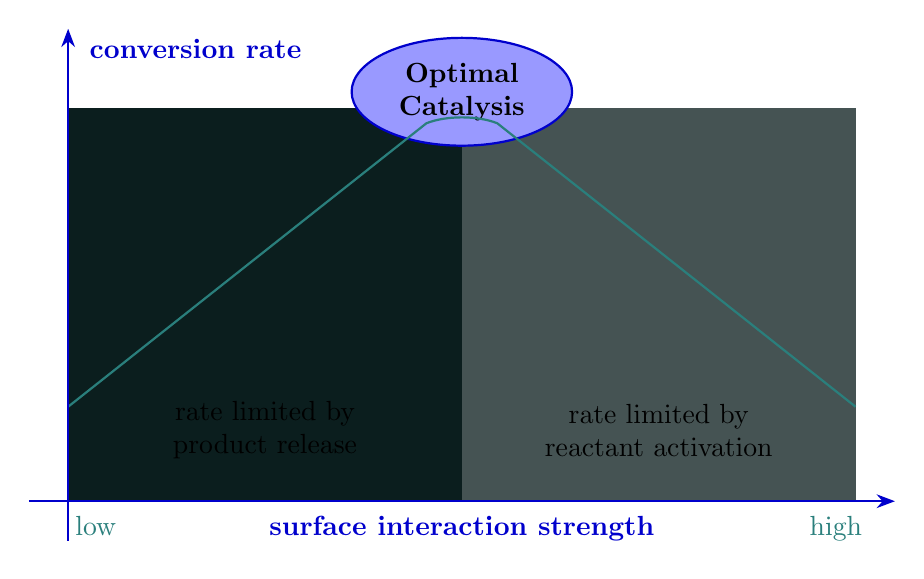
\begin{tikzpicture}[
    font=\rmfamily,
    axis/.style={-Stealth, thick, color=axisblue},
    label/.style={color=axisblue},
    volcano/.style={thick, color=plotgreen},
    oval_node/.style={
        ellipse,
        draw=ovalborder,
        fill=ovalfill,
        text=black,
        font=\bfseries,
        align=center,
        minimum height=1.1cm,
        minimum width=2.8cm,
        thick
    },
    region_text/.style={
        text=black,
        text width=3.5cm,
        align=center
    }
]

\definecolor{axisblue}{HTML}{0000CC}
\definecolor{plotgreen}{HTML}{2A7F7C}
\definecolor{bgleft}{HTML}{0B1E1E}
\definecolor{bgright}{HTML}{455353}
\definecolor{ovalfill}{HTML}{9999FF}
\definecolor{ovalborder}{HTML}{0000CC}

\def\xmax{10}
\def\ymax{5}
\def\xpeak{5}
\def\ypeak{5.2}
\def\yoval{5.2}

\fill[bgleft] (0,0) rectangle (\xpeak, \ymax);
\fill[bgright] (\xpeak,0) rectangle (\xmax, \ymax);

\node[oval_node] at (\xpeak, \yoval) {Optimal \\ Catalysis};

\draw[volcano] (0, 1.2) -- (4.55, 4.8) .. controls (4.8, 4.9) and (5.2, 4.9) .. (5.45, 4.8) -- (\xmax, 1.2);

\draw[axis] (-0.5, 0) -- (\xmax + 0.5, 0);
\draw[axis] (0, -0.5) -- (0, \ymax + 1);

\node[label, font=\bfseries, anchor=west] at (0.15, \ymax + 0.75) {conversion rate};
\node[label, font=\bfseries, below=2pt] at (\xpeak, 0) {surface interaction strength};
\node[color=plotgreen, below=2pt] at (0.35, 0) {low};
\node[color=plotgreen, below=2pt] at (9.75, 0) {high};

\node[region_text] at (2.5, 0.9) {rate limited by\\product release};
\node[region_text] at (7.5, 0.9) {rate limited by\\reactant activation};

\end{tikzpicture}
\end{document}